\documentclass[1p]{elsarticle_modified}
%\bibliographystyle{elsarticle-num}

%\usepackage[colorlinks]{hyperref}
%\usepackage{abbrmath_seonhwa} %\Abb, \Ascr, \Acal ,\Abf, \Afrak
\usepackage{amsfonts}
\usepackage{amssymb}
\usepackage{amsmath}
\usepackage{amsthm}
\usepackage{scalefnt}
\usepackage{amsbsy}
\usepackage{kotex}
\usepackage{caption}
\usepackage{subfig}
\usepackage{color}
\usepackage{graphicx}
\usepackage{xcolor} %% white, black, red, green, blue, cyan, magenta, yellow
\usepackage{float}
\usepackage{setspace}
\usepackage{hyperref}

\usepackage{tikz}
\usetikzlibrary{arrows}

\usepackage{multirow}
\usepackage{array} % fixed length table
\usepackage{hhline}

%%%%%%%%%%%%%%%%%%%%%
\makeatletter
\renewcommand*\env@matrix[1][\arraystretch]{%
	\edef\arraystretch{#1}%
	\hskip -\arraycolsep
	\let\@ifnextchar\new@ifnextchar
	\array{*\c@MaxMatrixCols c}}
\makeatother %https://tex.stackexchange.com/questions/14071/how-can-i-increase-the-line-spacing-in-a-matrix
%%%%%%%%%%%%%%%

\usepackage[normalem]{ulem}

\newcommand{\msout}[1]{\ifmmode\text{\sout{\ensuremath{#1}}}\else\sout{#1}\fi}
%SOURCE: \msout is \stkout macro in https://tex.stackexchange.com/questions/20609/strikeout-in-math-mode

\newcommand{\cancel}[1]{
	\ifmmode
	{\color{red}\msout{#1}}
	\else
	{\color{red}\sout{#1}}
	\fi
}

\newcommand{\add}[1]{
	{\color{blue}\uwave{#1}}
}

\newcommand{\replace}[2]{
	\ifmmode
	{\color{red}\msout{#1}}{\color{blue}\uwave{#2}}
	\else
	{\color{red}\sout{#1}}{\color{blue}\uwave{#2}}
	\fi
}

\newcommand{\Sol}{\mathcal{S}} %segment
\newcommand{\D}{D} %diagram
\newcommand{\A}{\mathcal{A}} %arc


%%%%%%%%%%%%%%%%%%%%%%%%%%%%%5 test

\def\sl{\operatorname{\textup{SL}}(2,\Cbb)}
\def\psl{\operatorname{\textup{PSL}}(2,\Cbb)}
\def\quan{\mkern 1mu \triangleright \mkern 1mu}

\theoremstyle{definition}
\newtheorem{thm}{Theorem}[section]
\newtheorem{prop}[thm]{Proposition}
\newtheorem{lem}[thm]{Lemma}
\newtheorem{ques}[thm]{Question}
\newtheorem{cor}[thm]{Corollary}
\newtheorem{defn}[thm]{Definition}
\newtheorem{exam}[thm]{Example}
\newtheorem{rmk}[thm]{Remark}
\newtheorem{alg}[thm]{Algorithm}

\newcommand{\I}{\sqrt{-1}}
\begin{document}

%\begin{frontmatter}
%
%\title{Boundary parabolic representations of knots up to 8 crossings}
%
%%% Group authors per affiliation:
%\author{Yunhi Cho} 
%\address{Department of Mathematics, University of Seoul, Seoul, Korea}
%\ead{yhcho@uos.ac.kr}
%
%
%\author{Seonhwa Kim} %\fnref{s_kim}}
%\address{Center for Geometry and Physics, Institute for Basic Science, Pohang, 37673, Korea}
%\ead{ryeona17@ibs.re.kr}
%
%\author{Hyuk Kim}
%\address{Department of Mathematical Sciences, Seoul National University, Seoul 08826, Korea}
%\ead{hyukkim@snu.ac.kr}
%
%\author{Seokbeom Yoon}
%\address{Department of Mathematical Sciences, Seoul National University, Seoul, 08826,  Korea}
%\ead{sbyoon15@snu.ac.kr}
%
%\begin{abstract}
%We find all boundary parabolic representation of knots up to 8 crossings.
%
%\end{abstract}
%\begin{keyword}
%    \MSC[2010] 57M25 
%\end{keyword}
%
%\end{frontmatter}

%\linenumbers
%\tableofcontents
%
\newcommand\colored[1]{\textcolor{white}{\rule[-0.35ex]{0.8em}{1.4ex}}\kern-0.8em\color{red} #1}%
%\newcommand\colored[1]{\textcolor{white}{ #1}\kern-2.17ex	\textcolor{white}{ #1}\kern-1.81ex	\textcolor{white}{ #1}\kern-2.15ex\color{red}#1	}

{\Large $\underline{11a_{39}~(K11a_{39})}$}

\setlength{\tabcolsep}{10pt}
\renewcommand{\arraystretch}{1.6}
\vspace{1cm}\begin{tabular}{m{100pt}>{\centering\arraybackslash}m{274pt}}
\multirow{5}{120pt}{
	\centering
	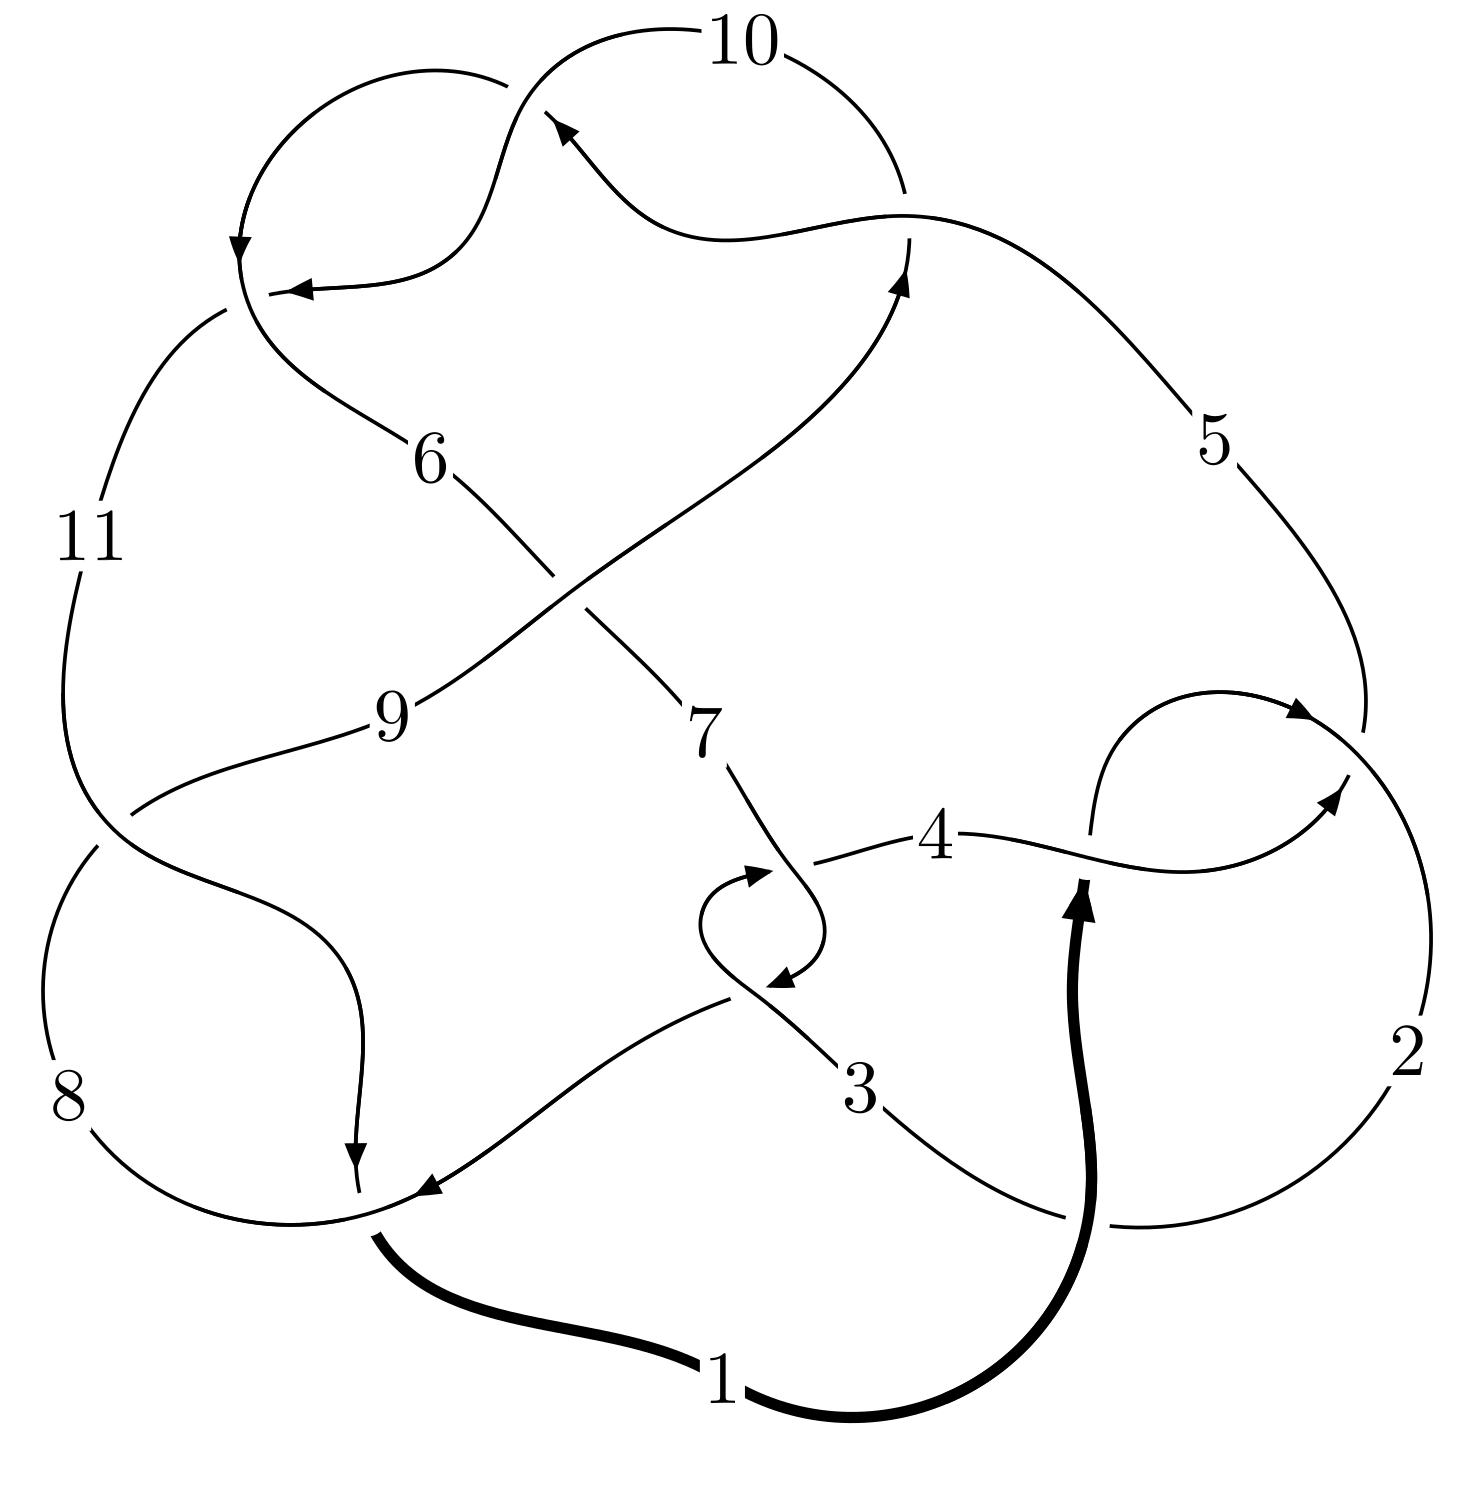
\includegraphics[width=112pt]{../../../GIT/diagram.site/Diagrams/png/288_11a_39.png}\\
\ \ \ A knot diagram\footnotemark}&
\allowdisplaybreaks
\textbf{Linearized knot diagam} \\
\cline{2-2}
 &
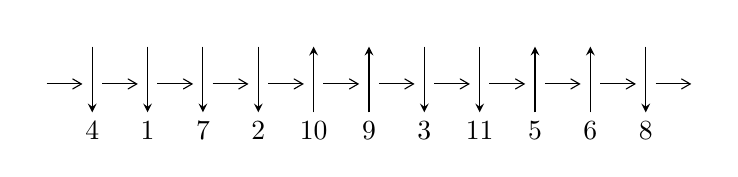
\begin{tikzpicture}[x=20pt, y=17pt]
	% nodes
	\node (C0) at (0, 0) {};
	\node (C1) at (1, 0) {};
	\node (C1U) at (1, +1) {};
	\node (C1D) at (1, -1) {4};

	\node (C2) at (2, 0) {};
	\node (C2U) at (2, +1) {};
	\node (C2D) at (2, -1) {1};

	\node (C3) at (3, 0) {};
	\node (C3U) at (3, +1) {};
	\node (C3D) at (3, -1) {7};

	\node (C4) at (4, 0) {};
	\node (C4U) at (4, +1) {};
	\node (C4D) at (4, -1) {2};

	\node (C5) at (5, 0) {};
	\node (C5U) at (5, +1) {};
	\node (C5D) at (5, -1) {10};

	\node (C6) at (6, 0) {};
	\node (C6U) at (6, +1) {};
	\node (C6D) at (6, -1) {9};

	\node (C7) at (7, 0) {};
	\node (C7U) at (7, +1) {};
	\node (C7D) at (7, -1) {3};

	\node (C8) at (8, 0) {};
	\node (C8U) at (8, +1) {};
	\node (C8D) at (8, -1) {11};

	\node (C9) at (9, 0) {};
	\node (C9U) at (9, +1) {};
	\node (C9D) at (9, -1) {5};

	\node (C10) at (10, 0) {};
	\node (C10U) at (10, +1) {};
	\node (C10D) at (10, -1) {6};

	\node (C11) at (11, 0) {};
	\node (C11U) at (11, +1) {};
	\node (C11D) at (11, -1) {8};
	\node (C12) at (12, 0) {};

	% arrows
	\draw[->,>={angle 60}]
	(C0) edge (C1) (C1) edge (C2) (C2) edge (C3) (C3) edge (C4) (C4) edge (C5) (C5) edge (C6) (C6) edge (C7) (C7) edge (C8) (C8) edge (C9) (C9) edge (C10) (C10) edge (C11) (C11) edge (C12) ;	\draw[->,>=stealth]
	(C1U) edge (C1D) (C2U) edge (C2D) (C3U) edge (C3D) (C4U) edge (C4D) (C5D) edge (C5U) (C6D) edge (C6U) (C7U) edge (C7D) (C8U) edge (C8D) (C9D) edge (C9U) (C10D) edge (C10U) (C11U) edge (C11D) ;
	\end{tikzpicture} \\
\hhline{~~} \\& 
\textbf{Solving Sequence} \\ \cline{2-2} 
 &
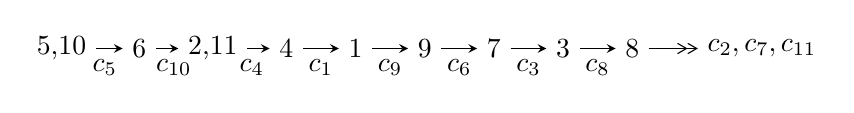
\begin{tikzpicture}[x=25pt, y=7pt]
	% node
	\node (A0) at (-1/8, 0) {5,10};
	\node (A1) at (1, 0) {6};
	\node (A2) at (33/16, 0) {2,11};
	\node (A3) at (25/8, 0) {4};
	\node (A4) at (33/8, 0) {1};
	\node (A5) at (41/8, 0) {9};
	\node (A6) at (49/8, 0) {7};
	\node (A7) at (57/8, 0) {3};
	\node (A8) at (65/8, 0) {8};
	\node (C1) at (1/2, -1) {$c_{5}$};
	\node (C2) at (3/2, -1) {$c_{10}$};
	\node (C3) at (21/8, -1) {$c_{4}$};
	\node (C4) at (29/8, -1) {$c_{1}$};
	\node (C5) at (37/8, -1) {$c_{9}$};
	\node (C6) at (45/8, -1) {$c_{6}$};
	\node (C7) at (53/8, -1) {$c_{3}$};
	\node (C8) at (61/8, -1) {$c_{8}$};
	\node (A9) at (10, 0) {$c_{2},c_{7},c_{11}$};

	% edge
	\draw[->,>=stealth]	
	(A0) edge (A1) (A1) edge (A2) (A2) edge (A3) (A3) edge (A4) (A4) edge (A5) (A5) edge (A6) (A6) edge (A7) (A7) edge (A8) ;
	\draw[->>,>={angle 60}]	
	(A8) edge (A9);
\end{tikzpicture} \\ 

\end{tabular} \\

\footnotetext{
The image of knot diagram is generated by the software ``\textbf{Draw programme}" developed by Andrew Bartholomew(\url{http://www.layer8.co.uk/maths/draw/index.htm\#Running-draw}), where we modified some parts for our purpose(\url{https://github.com/CATsTAILs/LinksPainter}).
}\phantom \\ \newline 
\centering \textbf{Ideals for irreducible components\footnotemark of $X_{\text{par}}$} 
 
\begin{align*}
I^u_{1}&=\langle 
u^{54}- u^{53}+\cdots+b-3 u,\;-2 u^{54}+2 u^{53}+\cdots+a+6 u,\;u^{55}-2 u^{54}+\cdots+2 u+1\rangle \\
I^u_{2}&=\langle 
b+1,\;u^3+a-2 u,\;u^5- u^4-2 u^3+u^2+u+1\rangle \\
\\
\end{align*}
\raggedright * 2 irreducible components of $\dim_{\mathbb{C}}=0$, with total 60 representations.\\
\footnotetext{All coefficients of polynomials are rational numbers. But the coefficients are sometimes approximated in decimal forms when there is not enough margin.}
\newpage
\renewcommand{\arraystretch}{1}
\centering \section*{I. $I^u_{1}= \langle u^{54}- u^{53}+\cdots+b-3 u,\;-2 u^{54}+2 u^{53}+\cdots+a+6 u,\;u^{55}-2 u^{54}+\cdots+2 u+1 \rangle$}
\flushleft \textbf{(i) Arc colorings}\\
\begin{tabular}{m{7pt} m{180pt} m{7pt} m{180pt} }
\flushright $a_{5}=$&$\begin{pmatrix}1\\0\end{pmatrix}$ \\
\flushright $a_{10}=$&$\begin{pmatrix}0\\u\end{pmatrix}$ \\
\flushright $a_{6}=$&$\begin{pmatrix}1\\- u^2\end{pmatrix}$ \\
\flushright $a_{2}=$&$\begin{pmatrix}2 u^{54}-2 u^{53}+\cdots+13 u^2-6 u\\- u^{54}+u^{53}+\cdots-2 u^2+3 u\end{pmatrix}$ \\
\flushright $a_{11}=$&$\begin{pmatrix}u\\- u^3+u\end{pmatrix}$ \\
\flushright $a_{4}=$&$\begin{pmatrix}u^{54}- u^{53}+\cdots-5 u+1\\- u^{54}+u^{53}+\cdots-3 u^2+2 u\end{pmatrix}$ \\
\flushright $a_{1}=$&$\begin{pmatrix}u^9-4 u^7+5 u^5-2 u^3+u\\- u^{11}+5 u^9-8 u^7+3 u^5+u^3+u\end{pmatrix}$ \\
\flushright $a_{9}=$&$\begin{pmatrix}- u\\u\end{pmatrix}$ \\
\flushright $a_{7}=$&$\begin{pmatrix}- u^4+u^2+1\\u^4-2 u^2\end{pmatrix}$ \\
\flushright $a_{3}=$&$\begin{pmatrix}3 u^{54}-3 u^{53}+\cdots+11 u^2-7 u\\- u^{54}+u^{53}+\cdots- u^2+3 u\end{pmatrix}$ \\
\flushright $a_{8}=$&$\begin{pmatrix}- u^5+2 u^3- u\\u^7-3 u^5+2 u^3+u\end{pmatrix}$\\ \flushright $a_{8}=$&$\begin{pmatrix}- u^5+2 u^3- u\\u^7-3 u^5+2 u^3+u\end{pmatrix}$\\&\end{tabular}
\flushleft \textbf{(ii) Obstruction class $= -1$}\\~\\
\flushleft \textbf{(iii) Cusp Shapes $= -2 u^{54}+4 u^{53}+\cdots+3 u-6$}\\~\\
\newpage\renewcommand{\arraystretch}{1}
\flushleft \textbf{(iv) u-Polynomials at the component}\newline \\
\begin{tabular}{m{50pt}|m{274pt}}
Crossings & \hspace{64pt}u-Polynomials at each crossing \\
\hline $$\begin{aligned}c_{1},c_{4}\end{aligned}$$&$\begin{aligned}
&u^{55}-6 u^{54}+\cdots-8 u+1
\end{aligned}$\\
\hline $$\begin{aligned}c_{2}\end{aligned}$$&$\begin{aligned}
&u^{55}+24 u^{54}+\cdots+8 u+1
\end{aligned}$\\
\hline $$\begin{aligned}c_{3},c_{7}\end{aligned}$$&$\begin{aligned}
&u^{55}+u^{54}+\cdots+64 u+32
\end{aligned}$\\
\hline $$\begin{aligned}c_{5},c_{9},c_{10}\end{aligned}$$&$\begin{aligned}
&u^{55}-2 u^{54}+\cdots+2 u+1
\end{aligned}$\\
\hline $$\begin{aligned}c_{6}\end{aligned}$$&$\begin{aligned}
&u^{55}+6 u^{54}+\cdots+302 u+77
\end{aligned}$\\
\hline $$\begin{aligned}c_{8},c_{11}\end{aligned}$$&$\begin{aligned}
&u^{55}-8 u^{54}+\cdots+94 u-7
\end{aligned}$\\
\hline
\end{tabular}\\~\\
\newpage\renewcommand{\arraystretch}{1}
\flushleft \textbf{(v) Riley Polynomials at the component}\newline \\
\begin{tabular}{m{50pt}|m{274pt}}
Crossings & \hspace{64pt}Riley Polynomials at each crossing \\
\hline $$\begin{aligned}c_{1},c_{4}\end{aligned}$$&$\begin{aligned}
&y^{55}-24 y^{54}+\cdots+8 y-1
\end{aligned}$\\
\hline $$\begin{aligned}c_{2}\end{aligned}$$&$\begin{aligned}
&y^{55}+20 y^{54}+\cdots-220 y-1
\end{aligned}$\\
\hline $$\begin{aligned}c_{3},c_{7}\end{aligned}$$&$\begin{aligned}
&y^{55}+33 y^{54}+\cdots-14848 y-1024
\end{aligned}$\\
\hline $$\begin{aligned}c_{5},c_{9},c_{10}\end{aligned}$$&$\begin{aligned}
&y^{55}-52 y^{54}+\cdots+14 y-1
\end{aligned}$\\
\hline $$\begin{aligned}c_{6}\end{aligned}$$&$\begin{aligned}
&y^{55}-20 y^{54}+\cdots+146490 y-5929
\end{aligned}$\\
\hline $$\begin{aligned}c_{8},c_{11}\end{aligned}$$&$\begin{aligned}
&y^{55}+48 y^{54}+\cdots+4314 y-49
\end{aligned}$\\
\hline
\end{tabular}\\~\\
\newpage\flushleft \textbf{(vi) Complex Volumes and Cusp Shapes}
$$\begin{array}{c|c|c}  
\text{Solutions to }I^u_{1}& \I (\text{vol} + \sqrt{-1}CS) & \text{Cusp shape}\\
 \hline 
\begin{aligned}
u &= \phantom{-}1.078520 + 0.133677 I \\
a &= \phantom{-}0.516431 + 0.026697 I \\
b &= \phantom{-}0.912992 + 0.503784 I\end{aligned}
 & \phantom{-}1.55049 - 1.99776 I & \phantom{-0.000000 } 0 \\ \hline\begin{aligned}
u &= \phantom{-}1.078520 - 0.133677 I \\
a &= \phantom{-}0.516431 - 0.026697 I \\
b &= \phantom{-}0.912992 - 0.503784 I\end{aligned}
 & \phantom{-}1.55049 + 1.99776 I & \phantom{-0.000000 } 0 \\ \hline\begin{aligned}
u &= -0.405577 + 0.698559 I \\
a &= \phantom{-}1.19426 - 1.95218 I \\
b &= \phantom{-}1.131320 + 0.693924 I\end{aligned}
 & \phantom{-}4.79235 - 10.53540 I & -0.79776 + 8.38025 I \\ \hline\begin{aligned}
u &= -0.405577 - 0.698559 I \\
a &= \phantom{-}1.19426 + 1.95218 I \\
b &= \phantom{-}1.131320 - 0.693924 I\end{aligned}
 & \phantom{-}4.79235 + 10.53540 I & -0.79776 - 8.38025 I \\ \hline\begin{aligned}
u &= -0.429702 + 0.678403 I \\
a &= -0.970506 + 0.157558 I \\
b &= \phantom{-}0.496725 - 0.933713 I\end{aligned}
 & \phantom{-}6.73070 - 4.57214 I & \phantom{-}1.95904 + 4.03979 I \\ \hline\begin{aligned}
u &= -0.429702 - 0.678403 I \\
a &= -0.970506 - 0.157558 I \\
b &= \phantom{-}0.496725 + 0.933713 I\end{aligned}
 & \phantom{-}6.73070 + 4.57214 I & \phantom{-}1.95904 - 4.03979 I \\ \hline\begin{aligned}
u &= -0.544877 + 0.580820 I \\
a &= -0.164386 + 0.526147 I \\
b &= \phantom{-}1.103900 - 0.704264 I\end{aligned}
 & \phantom{-}5.32499 + 6.24906 I & \phantom{-}0.59828 - 2.50741 I \\ \hline\begin{aligned}
u &= -0.544877 - 0.580820 I \\
a &= -0.164386 - 0.526147 I \\
b &= \phantom{-}1.103900 + 0.704264 I\end{aligned}
 & \phantom{-}5.32499 - 6.24906 I & \phantom{-}0.59828 + 2.50741 I \\ \hline\begin{aligned}
u &= -0.510509 + 0.609052 I \\
a &= \phantom{-}0.325943 - 1.106180 I \\
b &= \phantom{-}0.541319 + 0.917635 I\end{aligned}
 & \phantom{-}7.04434 + 0.29231 I & \phantom{-}2.77654 + 2.24461 I \\ \hline\begin{aligned}
u &= -0.510509 - 0.609052 I \\
a &= \phantom{-}0.325943 + 1.106180 I \\
b &= \phantom{-}0.541319 - 0.917635 I\end{aligned}
 & \phantom{-}7.04434 - 0.29231 I & \phantom{-}2.77654 - 2.24461 I\\
 \hline 
 \end{array}$$\newpage$$\begin{array}{c|c|c}  
\text{Solutions to }I^u_{1}& \I (\text{vol} + \sqrt{-1}CS) & \text{Cusp shape}\\
 \hline 
\begin{aligned}
u &= \phantom{-}0.412834 + 0.641001 I \\
a &= -0.42450 - 2.15007 I \\
b &= -0.881787 + 0.589772 I\end{aligned}
 & \phantom{-}1.48241 + 4.33310 I & -1.64326 - 6.16138 I \\ \hline\begin{aligned}
u &= \phantom{-}0.412834 - 0.641001 I \\
a &= -0.42450 + 2.15007 I \\
b &= -0.881787 - 0.589772 I\end{aligned}
 & \phantom{-}1.48241 - 4.33310 I & -1.64326 + 6.16138 I \\ \hline\begin{aligned}
u &= \phantom{-}0.458268 + 0.584600 I \\
a &= \phantom{-}0.817122 + 0.781457 I \\
b &= -0.813432 - 0.582817 I\end{aligned}
 & \phantom{-}1.70221 - 0.32794 I & -0.771677 - 0.468923 I \\ \hline\begin{aligned}
u &= \phantom{-}0.458268 - 0.584600 I \\
a &= \phantom{-}0.817122 - 0.781457 I \\
b &= -0.813432 + 0.582817 I\end{aligned}
 & \phantom{-}1.70221 + 0.32794 I & -0.771677 + 0.468923 I \\ \hline\begin{aligned}
u &= -0.415395 + 0.603187 I \\
a &= -0.756841 + 1.109310 I \\
b &= -1.302130 + 0.031330 I\end{aligned}
 & \phantom{-}0.07504 - 1.93289 I & -0.05787 + 3.96687 I \\ \hline\begin{aligned}
u &= -0.415395 - 0.603187 I \\
a &= -0.756841 - 1.109310 I \\
b &= -1.302130 - 0.031330 I\end{aligned}
 & \phantom{-}0.07504 + 1.93289 I & -0.05787 - 3.96687 I \\ \hline\begin{aligned}
u &= -1.265410 + 0.116454 I \\
a &= -0.756900 - 0.079067 I \\
b &= -1.162780 + 0.205267 I\end{aligned}
 & \phantom{-}0.59955 - 1.29811 I & \phantom{-0.000000 } 0 \\ \hline\begin{aligned}
u &= -1.265410 - 0.116454 I \\
a &= -0.756900 + 0.079067 I \\
b &= -1.162780 - 0.205267 I\end{aligned}
 & \phantom{-}0.59955 + 1.29811 I & \phantom{-0.000000 } 0 \\ \hline\begin{aligned}
u &= \phantom{-}1.297170 + 0.044309 I \\
a &= \phantom{-}1.149320 + 0.636439 I \\
b &= -0.351487 - 0.343411 I\end{aligned}
 & \phantom{-}2.99828 + 0.14721 I & \phantom{-0.000000 } 0 \\ \hline\begin{aligned}
u &= \phantom{-}1.297170 - 0.044309 I \\
a &= \phantom{-}1.149320 - 0.636439 I \\
b &= -0.351487 + 0.343411 I\end{aligned}
 & \phantom{-}2.99828 - 0.14721 I & \phantom{-0.000000 } 0\\
 \hline 
 \end{array}$$\newpage$$\begin{array}{c|c|c}  
\text{Solutions to }I^u_{1}& \I (\text{vol} + \sqrt{-1}CS) & \text{Cusp shape}\\
 \hline 
\begin{aligned}
u &= \phantom{-}1.288550 + 0.158962 I \\
a &= -0.51700 - 2.28808 I \\
b &= -1.022630 + 0.390914 I\end{aligned}
 & \phantom{-}1.08244 + 3.51008 I & \phantom{-0.000000 } 0 \\ \hline\begin{aligned}
u &= \phantom{-}1.288550 - 0.158962 I \\
a &= -0.51700 + 2.28808 I \\
b &= -1.022630 - 0.390914 I\end{aligned}
 & \phantom{-}1.08244 - 3.51008 I & \phantom{-0.000000 } 0 \\ \hline\begin{aligned}
u &= -1.292250 + 0.245052 I \\
a &= \phantom{-}0.94579 - 1.66072 I \\
b &= \phantom{-}1.053490 + 0.579410 I\end{aligned}
 & \phantom{-}3.09735 - 8.51931 I & \phantom{-0.000000 } 0 \\ \hline\begin{aligned}
u &= -1.292250 - 0.245052 I \\
a &= \phantom{-}0.94579 + 1.66072 I \\
b &= \phantom{-}1.053490 - 0.579410 I\end{aligned}
 & \phantom{-}3.09735 + 8.51931 I & \phantom{-0.000000 } 0 \\ \hline\begin{aligned}
u &= \phantom{-}0.659363 + 0.177799 I \\
a &= \phantom{-}0.370767 + 0.659351 I \\
b &= \phantom{-}0.825967 - 0.561444 I\end{aligned}
 & \phantom{-}1.63950 + 2.24198 I & \phantom{-}1.57550 - 4.32492 I \\ \hline\begin{aligned}
u &= \phantom{-}0.659363 - 0.177799 I \\
a &= \phantom{-}0.370767 - 0.659351 I \\
b &= \phantom{-}0.825967 + 0.561444 I\end{aligned}
 & \phantom{-}1.63950 - 2.24198 I & \phantom{-}1.57550 + 4.32492 I \\ \hline\begin{aligned}
u &= \phantom{-}0.108922 + 0.669976 I \\
a &= \phantom{-}2.05168 + 0.39909 I \\
b &= \phantom{-}0.999297 - 0.553816 I\end{aligned}
 & -1.25442 + 5.19790 I & -5.46768 - 6.87562 I \\ \hline\begin{aligned}
u &= \phantom{-}0.108922 - 0.669976 I \\
a &= \phantom{-}2.05168 - 0.39909 I \\
b &= \phantom{-}0.999297 + 0.553816 I\end{aligned}
 & -1.25442 - 5.19790 I & -5.46768 + 6.87562 I \\ \hline\begin{aligned}
u &= \phantom{-}0.223843 + 0.635800 I \\
a &= \phantom{-}0.619795 + 0.836958 I \\
b &= \phantom{-}0.682905 + 0.426557 I\end{aligned}
 & -0.093506 + 0.957018 I & -1.47250 - 1.22419 I \\ \hline\begin{aligned}
u &= \phantom{-}0.223843 - 0.635800 I \\
a &= \phantom{-}0.619795 - 0.836958 I \\
b &= \phantom{-}0.682905 - 0.426557 I\end{aligned}
 & -0.093506 - 0.957018 I & -1.47250 + 1.22419 I\\
 \hline 
 \end{array}$$\newpage$$\begin{array}{c|c|c}  
\text{Solutions to }I^u_{1}& \I (\text{vol} + \sqrt{-1}CS) & \text{Cusp shape}\\
 \hline 
\begin{aligned}
u &= -1.345750 + 0.196757 I \\
a &= -0.348002 + 0.275917 I \\
b &= \phantom{-}0.325642 - 0.591557 I\end{aligned}
 & \phantom{-}4.93016 - 3.86526 I & \phantom{-0.000000 } 0 \\ \hline\begin{aligned}
u &= -1.345750 - 0.196757 I \\
a &= -0.348002 - 0.275917 I \\
b &= \phantom{-}0.325642 + 0.591557 I\end{aligned}
 & \phantom{-}4.93016 + 3.86526 I & \phantom{-0.000000 } 0 \\ \hline\begin{aligned}
u &= -1.39666 + 0.23010 I \\
a &= -0.011407 - 0.386009 I \\
b &= \phantom{-}0.636512 - 0.224540 I\end{aligned}
 & \phantom{-}5.07190 - 4.05462 I & \phantom{-0.000000 } 0 \\ \hline\begin{aligned}
u &= -1.39666 - 0.23010 I \\
a &= -0.011407 + 0.386009 I \\
b &= \phantom{-}0.636512 + 0.224540 I\end{aligned}
 & \phantom{-}5.07190 + 4.05462 I & \phantom{-0.000000 } 0 \\ \hline\begin{aligned}
u &= -1.43083 + 0.02750 I \\
a &= -0.66190 - 1.48550 I \\
b &= \phantom{-}0.838321 + 0.728876 I\end{aligned}
 & \phantom{-}7.99304 - 2.76322 I & \phantom{-0.000000 } 0 \\ \hline\begin{aligned}
u &= -1.43083 - 0.02750 I \\
a &= -0.66190 + 1.48550 I \\
b &= \phantom{-}0.838321 - 0.728876 I\end{aligned}
 & \phantom{-}7.99304 + 2.76322 I & \phantom{-0.000000 } 0 \\ \hline\begin{aligned}
u &= \phantom{-}0.220263 + 0.502370 I \\
a &= \phantom{-}0.543936 + 0.221214 I \\
b &= \phantom{-}0.182425 + 0.252129 I\end{aligned}
 & -0.008201 + 1.198200 I & -0.25143 - 5.38204 I \\ \hline\begin{aligned}
u &= \phantom{-}0.220263 - 0.502370 I \\
a &= \phantom{-}0.543936 - 0.221214 I \\
b &= \phantom{-}0.182425 - 0.252129 I\end{aligned}
 & -0.008201 - 1.198200 I & -0.25143 + 5.38204 I \\ \hline\begin{aligned}
u &= -0.046404 + 0.536106 I \\
a &= -2.41342 + 1.29245 I \\
b &= -1.047030 - 0.274962 I\end{aligned}
 & -3.02612 - 0.98819 I & -10.81757 + 0.62676 I \\ \hline\begin{aligned}
u &= -0.046404 - 0.536106 I \\
a &= -2.41342 - 1.29245 I \\
b &= -1.047030 + 0.274962 I\end{aligned}
 & -3.02612 + 0.98819 I & -10.81757 - 0.62676 I\\
 \hline 
 \end{array}$$\newpage$$\begin{array}{c|c|c}  
\text{Solutions to }I^u_{1}& \I (\text{vol} + \sqrt{-1}CS) & \text{Cusp shape}\\
 \hline 
\begin{aligned}
u &= \phantom{-}1.45734 + 0.22515 I \\
a &= \phantom{-}0.507704 - 0.942507 I \\
b &= -1.341850 - 0.047444 I\end{aligned}
 & \phantom{-}6.09964 + 4.98197 I & \phantom{-0.000000 } 0 \\ \hline\begin{aligned}
u &= \phantom{-}1.45734 - 0.22515 I \\
a &= \phantom{-}0.507704 + 0.942507 I \\
b &= -1.341850 + 0.047444 I\end{aligned}
 & \phantom{-}6.09964 - 4.98197 I & \phantom{-0.000000 } 0 \\ \hline\begin{aligned}
u &= -1.46520 + 0.21259 I \\
a &= \phantom{-}1.47883 - 1.30859 I \\
b &= -0.786253 + 0.638767 I\end{aligned}
 & \phantom{-}7.88540 - 2.59431 I & \phantom{-0.000000 } 0 \\ \hline\begin{aligned}
u &= -1.46520 - 0.21259 I \\
a &= \phantom{-}1.47883 + 1.30859 I \\
b &= -0.786253 - 0.638767 I\end{aligned}
 & \phantom{-}7.88540 + 2.59431 I & \phantom{-0.000000 } 0 \\ \hline\begin{aligned}
u &= -1.46151 + 0.23703 I \\
a &= \phantom{-}0.35860 + 2.60378 I \\
b &= -0.903696 - 0.627740 I\end{aligned}
 & \phantom{-}7.52118 - 7.54900 I & \phantom{-0.000000 } 0 \\ \hline\begin{aligned}
u &= -1.46151 - 0.23703 I \\
a &= \phantom{-}0.35860 - 2.60378 I \\
b &= -0.903696 + 0.627740 I\end{aligned}
 & \phantom{-}7.52118 + 7.54900 I & \phantom{-0.000000 } 0 \\ \hline\begin{aligned}
u &= \phantom{-}1.46676 + 0.25976 I \\
a &= \phantom{-}0.13179 + 2.56805 I \\
b &= \phantom{-}1.150220 - 0.701224 I\end{aligned}
 & \phantom{-}10.8274 + 14.0334 I & \phantom{-0.000000 } 0 \\ \hline\begin{aligned}
u &= \phantom{-}1.46676 - 0.25976 I \\
a &= \phantom{-}0.13179 - 2.56805 I \\
b &= \phantom{-}1.150220 + 0.701224 I\end{aligned}
 & \phantom{-}10.8274 - 14.0334 I & \phantom{-0.000000 } 0 \\ \hline\begin{aligned}
u &= \phantom{-}1.47287 + 0.24797 I \\
a &= -1.38353 - 1.05356 I \\
b &= \phantom{-}0.483891 + 0.966514 I\end{aligned}
 & \phantom{-}12.8723 + 7.9548 I & \phantom{-0.000000 } 0 \\ \hline\begin{aligned}
u &= \phantom{-}1.47287 - 0.24797 I \\
a &= -1.38353 + 1.05356 I \\
b &= \phantom{-}0.483891 - 0.966514 I\end{aligned}
 & \phantom{-}12.8723 - 7.9548 I & \phantom{-0.000000 } 0\\
 \hline 
 \end{array}$$\newpage$$\begin{array}{c|c|c}  
\text{Solutions to }I^u_{1}& \I (\text{vol} + \sqrt{-1}CS) & \text{Cusp shape}\\
 \hline 
\begin{aligned}
u &= \phantom{-}1.48811 + 0.18811 I \\
a &= -1.12025 - 1.22948 I \\
b &= \phantom{-}1.099520 + 0.737359 I\end{aligned}
 & \phantom{-}11.90410 - 3.49537 I & \phantom{-0.000000 } 0 \\ \hline\begin{aligned}
u &= \phantom{-}1.48811 - 0.18811 I \\
a &= -1.12025 + 1.22948 I \\
b &= \phantom{-}1.099520 - 0.737359 I\end{aligned}
 & \phantom{-}11.90410 + 3.49537 I & \phantom{-0.000000 } 0 \\ \hline\begin{aligned}
u &= \phantom{-}1.48611 + 0.20604 I \\
a &= -0.20805 + 1.92611 I \\
b &= \phantom{-}0.576460 - 0.947356 I\end{aligned}
 & \phantom{-}13.50700 + 2.65879 I & \phantom{-0.000000 } 0 \\ \hline\begin{aligned}
u &= \phantom{-}1.48611 - 0.20604 I \\
a &= -0.20805 - 1.92611 I \\
b &= \phantom{-}0.576460 + 0.947356 I\end{aligned}
 & \phantom{-}13.50700 - 2.65879 I & \phantom{-0.000000 } 0 \\ \hline\begin{aligned}
u &= -0.217641\phantom{ +0.000000I} \\
a &= \phantom{-}2.44944\phantom{ +0.000000I} \\
b &= -0.855618\phantom{ +0.000000I}\end{aligned}
 & -1.24884\phantom{ +0.000000I} & -7.99830\phantom{ +0.000000I}\\
 \hline 
 \end{array}$$\newpage\newpage\renewcommand{\arraystretch}{1}
\centering \section*{II. $I^u_{2}= \langle b+1,\;u^3+a-2 u,\;u^5- u^4-2 u^3+u^2+u+1 \rangle$}
\flushleft \textbf{(i) Arc colorings}\\
\begin{tabular}{m{7pt} m{180pt} m{7pt} m{180pt} }
\flushright $a_{5}=$&$\begin{pmatrix}1\\0\end{pmatrix}$ \\
\flushright $a_{10}=$&$\begin{pmatrix}0\\u\end{pmatrix}$ \\
\flushright $a_{6}=$&$\begin{pmatrix}1\\- u^2\end{pmatrix}$ \\
\flushright $a_{2}=$&$\begin{pmatrix}- u^3+2 u\\-1\end{pmatrix}$ \\
\flushright $a_{11}=$&$\begin{pmatrix}u\\- u^3+u\end{pmatrix}$ \\
\flushright $a_{4}=$&$\begin{pmatrix}- u^3+2 u+1\\-1\end{pmatrix}$ \\
\flushright $a_{1}=$&$\begin{pmatrix}-1\\0\end{pmatrix}$ \\
\flushright $a_{9}=$&$\begin{pmatrix}- u\\u\end{pmatrix}$ \\
\flushright $a_{7}=$&$\begin{pmatrix}- u^4+u^2+1\\u^4-2 u^2\end{pmatrix}$ \\
\flushright $a_{3}=$&$\begin{pmatrix}- u^3+2 u+1\\-1\end{pmatrix}$ \\
\flushright $a_{8}=$&$\begin{pmatrix}- u^4+u^2+1\\u^4-2 u^2\end{pmatrix}$\\ \flushright $a_{8}=$&$\begin{pmatrix}- u^4+u^2+1\\u^4-2 u^2\end{pmatrix}$\\&\end{tabular}
\flushleft \textbf{(ii) Obstruction class $= 1$}\\~\\
\flushleft \textbf{(iii) Cusp Shapes $= -5 u^3+u^2+8 u-3$}\\~\\
\newpage\renewcommand{\arraystretch}{1}
\flushleft \textbf{(iv) u-Polynomials at the component}\newline \\
\begin{tabular}{m{50pt}|m{274pt}}
Crossings & \hspace{64pt}u-Polynomials at each crossing \\
\hline $$\begin{aligned}c_{1}\end{aligned}$$&$\begin{aligned}
&(u-1)^5
\end{aligned}$\\
\hline $$\begin{aligned}c_{2},c_{4}\end{aligned}$$&$\begin{aligned}
&(u+1)^5
\end{aligned}$\\
\hline $$\begin{aligned}c_{3},c_{7}\end{aligned}$$&$\begin{aligned}
&u^5
\end{aligned}$\\
\hline $$\begin{aligned}c_{5}\end{aligned}$$&$\begin{aligned}
&u^5- u^4-2 u^3+u^2+u+1
\end{aligned}$\\
\hline $$\begin{aligned}c_{6}\end{aligned}$$&$\begin{aligned}
&u^5+3 u^4+4 u^3+u^2- u-1
\end{aligned}$\\
\hline $$\begin{aligned}c_{8}\end{aligned}$$&$\begin{aligned}
&u^5+u^4+2 u^3+u^2+u+1
\end{aligned}$\\
\hline $$\begin{aligned}c_{9},c_{10}\end{aligned}$$&$\begin{aligned}
&u^5+u^4-2 u^3- u^2+u-1
\end{aligned}$\\
\hline $$\begin{aligned}c_{11}\end{aligned}$$&$\begin{aligned}
&u^5- u^4+2 u^3- u^2+u-1
\end{aligned}$\\
\hline
\end{tabular}\\~\\
\newpage\renewcommand{\arraystretch}{1}
\flushleft \textbf{(v) Riley Polynomials at the component}\newline \\
\begin{tabular}{m{50pt}|m{274pt}}
Crossings & \hspace{64pt}Riley Polynomials at each crossing \\
\hline $$\begin{aligned}c_{1},c_{2},c_{4}\end{aligned}$$&$\begin{aligned}
&(y-1)^5
\end{aligned}$\\
\hline $$\begin{aligned}c_{3},c_{7}\end{aligned}$$&$\begin{aligned}
&y^5
\end{aligned}$\\
\hline $$\begin{aligned}c_{5},c_{9},c_{10}\end{aligned}$$&$\begin{aligned}
&y^5-5 y^4+8 y^3-3 y^2- y-1
\end{aligned}$\\
\hline $$\begin{aligned}c_{6}\end{aligned}$$&$\begin{aligned}
&y^5- y^4+8 y^3-3 y^2+3 y-1
\end{aligned}$\\
\hline $$\begin{aligned}c_{8},c_{11}\end{aligned}$$&$\begin{aligned}
&y^5+3 y^4+4 y^3+y^2- y-1
\end{aligned}$\\
\hline
\end{tabular}\\~\\
\newpage\flushleft \textbf{(vi) Complex Volumes and Cusp Shapes}
$$\begin{array}{c|c|c}  
\text{Solutions to }I^u_{2}& \I (\text{vol} + \sqrt{-1}CS) & \text{Cusp shape}\\
 \hline 
\begin{aligned}
u &= -1.21774\phantom{ +0.000000I} \\
a &= -0.629714\phantom{ +0.000000I} \\
b &= -1.00000\phantom{ +0.000000I}\end{aligned}
 & \phantom{-}0.756147\phantom{ +0.000000I} & -2.23020\phantom{ +0.000000I} \\ \hline\begin{aligned}
u &= -0.309916 + 0.549911 I \\
a &= -0.871221 + 1.107660 I \\
b &= -1.00000\phantom{ +0.000000I}\end{aligned}
 & -1.31583 - 1.53058 I & -6.94263 + 4.09764 I \\ \hline\begin{aligned}
u &= -0.309916 - 0.549911 I \\
a &= -0.871221 - 1.107660 I \\
b &= -1.00000\phantom{ +0.000000I}\end{aligned}
 & -1.31583 + 1.53058 I & -6.94263 - 4.09764 I \\ \hline\begin{aligned}
u &= \phantom{-}1.41878 + 0.21917 I \\
a &= \phantom{-}0.186078 - 0.874646 I \\
b &= -1.00000\phantom{ +0.000000I}\end{aligned}
 & \phantom{-}4.22763 + 4.40083 I & -2.94226 - 4.18967 I \\ \hline\begin{aligned}
u &= \phantom{-}1.41878 - 0.21917 I \\
a &= \phantom{-}0.186078 + 0.874646 I \\
b &= -1.00000\phantom{ +0.000000I}\end{aligned}
 & \phantom{-}4.22763 - 4.40083 I & -2.94226 + 4.18967 I\\
 \hline 
 \end{array}$$\newpage
\newpage\renewcommand{\arraystretch}{1}
\centering \section*{ III. u-Polynomials}
\begin{tabular}{m{50pt}|m{274pt}}
Crossings & \hspace{64pt}u-Polynomials at each crossing \\
\hline $$\begin{aligned}c_{1}\end{aligned}$$&$\begin{aligned}
&((u-1)^5)(u^{55}-6 u^{54}+\cdots-8 u+1)
\end{aligned}$\\
\hline $$\begin{aligned}c_{2}\end{aligned}$$&$\begin{aligned}
&((u+1)^5)(u^{55}+24 u^{54}+\cdots+8 u+1)
\end{aligned}$\\
\hline $$\begin{aligned}c_{3},c_{7}\end{aligned}$$&$\begin{aligned}
&u^5(u^{55}+u^{54}+\cdots+64 u+32)
\end{aligned}$\\
\hline $$\begin{aligned}c_{4}\end{aligned}$$&$\begin{aligned}
&((u+1)^5)(u^{55}-6 u^{54}+\cdots-8 u+1)
\end{aligned}$\\
\hline $$\begin{aligned}c_{5}\end{aligned}$$&$\begin{aligned}
&(u^5- u^4-2 u^3+u^2+u+1)(u^{55}-2 u^{54}+\cdots+2 u+1)
\end{aligned}$\\
\hline $$\begin{aligned}c_{6}\end{aligned}$$&$\begin{aligned}
&(u^5+3 u^4+4 u^3+u^2- u-1)(u^{55}+6 u^{54}+\cdots+302 u+77)
\end{aligned}$\\
\hline $$\begin{aligned}c_{8}\end{aligned}$$&$\begin{aligned}
&(u^5+u^4+2 u^3+u^2+u+1)(u^{55}-8 u^{54}+\cdots+94 u-7)
\end{aligned}$\\
\hline $$\begin{aligned}c_{9},c_{10}\end{aligned}$$&$\begin{aligned}
&(u^5+u^4-2 u^3- u^2+u-1)(u^{55}-2 u^{54}+\cdots+2 u+1)
\end{aligned}$\\
\hline $$\begin{aligned}c_{11}\end{aligned}$$&$\begin{aligned}
&(u^5- u^4+2 u^3- u^2+u-1)(u^{55}-8 u^{54}+\cdots+94 u-7)
\end{aligned}$\\
\hline
\end{tabular}\newpage\renewcommand{\arraystretch}{1}
\centering \section*{ IV. Riley Polynomials}
\begin{tabular}{m{50pt}|m{274pt}}
Crossings & \hspace{64pt}Riley Polynomials at each crossing \\
\hline $$\begin{aligned}c_{1},c_{4}\end{aligned}$$&$\begin{aligned}
&((y-1)^5)(y^{55}-24 y^{54}+\cdots+8 y-1)
\end{aligned}$\\
\hline $$\begin{aligned}c_{2}\end{aligned}$$&$\begin{aligned}
&((y-1)^5)(y^{55}+20 y^{54}+\cdots-220 y-1)
\end{aligned}$\\
\hline $$\begin{aligned}c_{3},c_{7}\end{aligned}$$&$\begin{aligned}
&y^5(y^{55}+33 y^{54}+\cdots-14848 y-1024)
\end{aligned}$\\
\hline $$\begin{aligned}c_{5},c_{9},c_{10}\end{aligned}$$&$\begin{aligned}
&(y^5-5 y^4+8 y^3-3 y^2- y-1)(y^{55}-52 y^{54}+\cdots+14 y-1)
\end{aligned}$\\
\hline $$\begin{aligned}c_{6}\end{aligned}$$&$\begin{aligned}
&(y^5- y^4+8 y^3-3 y^2+3 y-1)(y^{55}-20 y^{54}+\cdots+146490 y-5929)
\end{aligned}$\\
\hline $$\begin{aligned}c_{8},c_{11}\end{aligned}$$&$\begin{aligned}
&(y^5+3 y^4+4 y^3+y^2- y-1)(y^{55}+48 y^{54}+\cdots+4314 y-49)
\end{aligned}$\\
\hline
\end{tabular}
\vskip 2pc
\end{document}